\chapter{Modelo} %#{{{1
%#{{{2
\begin{epigraphs}
\qitem{ Every attempt to employ mathematical methods in the study of chemical
questions must be considered profoundly irrational and contrary to the spirit
of chemistry.... if mathematical analysis should ever hold a prominent
place in chemistry -- an aberration which is happily almost impossible --
it would occasion a rapid and widespread degeneration of that science.}
{\---- \textsc{Auguste Comte, 1798-1857}}
\end{epigraphs}

Este trabalho é uma extensão do modelo que foi inicialmente apresentado
por  Caticha e Vicente \cite{Caticha2011a} para o estudo da dinâmica
moral da sociedade. O trabalho de Caticha e Vicente é descrito de forma
mais detalhada e dentro do contexto mais geral de dinâmica de opinião no
apêndice \ref{sec:plandia}, onde também apresentamos algumas modificações
e cenários de simulação trabalhados durante o período de doutoramento.

No modelo, um  agente $i$ representa a \textbf{matriz moral} de uma pessoa 
através de um vetor $\bm \omega_i = (\omega_{i 1},\ldots,\omega_{i 5})$
de 5 dimensões, onde cada componente $\omega_{i a}$ pode ser interpretada
como uma dimensão moral.  Assumimos, por simplicidade, que as pessoas
são igualmente morais, ou seja, a diferença entre morais de indivíduos é
expressa somente através da direção no espaço moral. Para isso, faremos que
os vetores morais de nossos agentes sejam unitários ($|\bm \omega_i| = 1$).

Uma das hipóteses mais fortes do nosso trabalho é que a descrição
matemática do aprendizado moral pode ser dividida em duas fases, sendo que
cada uma das fases necessita de modelagens de distintas. A \textbf{fase 1}
mimetiza o aprendizado moral de pessoas no período da infância até a
adolescência. Durante essa fase o julgamento de assuntos com conteúdo moral
muda a estratégia cognitiva do agente. Já na \textbf{fase 2}, representamos
o aprendizado moral de indivíduos adultos, ou de indivíduos que já tem
uma estratégia cognitiva estabilizada. Nessa fase, estamos interessados
nos estados estacionários e nos mecanismos de controle da dinâmica de
opiniões da sociedade.

Em ambas as fases um agente $i$ modifica sua matriz moral ao receber
informações através da interação social com outro um agente $j$.
A interação social se dá através da discussão de assuntos com conteúdo
moral, onde a informação recebida pelo agente $i$ ao interagir com o
agente $j$  é escrita na forma $y_\mu=(\sigma_{j\mu},\bm x_\mu)$. Chamamos
de \textbf{assunto} os vetores $\bm x_\mu = (x_{\mu 1},\ldots,x_{\mu 5})$,
onde suas componentes representam o peso ou conteúdo de um fundamento moral
de um assunto discutido entre duas pessoas numa sociedade real.  O termo
$\sigma_{j\mu} = \pm 1$  é a \textbf{classificação}  que o agente $j$
dá ao assunto -- positiva/negativa ou favorável/contrario.

Como foi discutido no capítulo \ref{chap:mft}, esperamos que julgamentos
morais sejam feitos de maneira rápida e intuitiva. Para tanto, faremos com
que a classificação que o agente dá a um assunto seja feita pelo sinal
do produto escalar entre os vetores da matriz moral do agente e do conteúdo
moral do assunto, ou seja, $\sigma_{j \mu} = \mathrm sign ( h_{j \mu})$ onde
$h_{j \mu} = \bm \omega_j\cdot \bm x_\mu = \sum_{a=1}^5 \omega_{j a}x_{\mu
a}$. O termo $h_{j\mu}$ é o peso da classificação ou \textbf{opinião}
do agente em relação ao assunto discutido. Outra importante variável é
$z_\mu = h_{i\mu}\sigma_{j\mu}$ que expressa a concordância que o agente $i$
tem em relação a classificação do agente $j$ sobre o assunto $\mu$.

A troca de informação entre os agentes do modelo proposto por Caticha
e Vicente\citep{Caticha2011a} ocorre de maneira similar, no entanto,
a diferença fundamental entre esse modelo e o apresentado no presente
trabalho é que no primeiro não existe nenhum mecanismo de construção da
estratégia cognitiva do agente, o que faz com que ele só tenha uma fase
de aprendizado, que é similar a segunda fase de nossa modelagem.

\section{Fase 1: Criação de estratégia cognitiva} %#{{{2
\label{sec:ecog}

Durante a fase 1 o agente definirá sua estratégia cognitiva através de
trocas de informações com seus parceiros sociais. Como já discutimos
anteriormente, o agente interage com seus parceiros sociais e obtém
informações com conteúdo moral na forma $(\bm x_\mu, \sigma_\mu)$. Tendo
em vista que o agente recebe esse tipo de informação, iremos fazer uma
descrição probabilística de seu aprendizado usando algoritmo de aprendizado
Bayesiano aproximado, já que esse respeita critérios de razoabilidade. No
apêndice \ref{chap:apbayes}, apresentamos a motivação geral para o uso
de descrições probabilísticas assim como a dedução das equações do
aprendizado Bayesiano.

Sobre o ponto de vista de psicologia, podemos interpretar o algorítmo
Bayesiano como uma descrição motivacional do aprendizado, no qual o agente é
motivado a aprender para diminuir um custo psicológico $\mathcal E$. Outra
interpretação equivalente pode ser feita sobre a perspectiva de aprendizado
por reforço, onde através de um algoritmo do tipo Hebbiano\footnote{A
ideia de aprendizado Hebbiano é descrita no apêndice \ref{chap:neuro}},
o indivíduo responde de acordo com um protocolo automático interno
representado por uma função $F$ de modulação do aprendizado\footnote{
Podemos observar pela equação \ref{eq:F1} que a função de modulação
e o custo psicológicos estão relacionados através da expressão $F =
-C\partial_z \mathcal E $. }.  O formato da função de modulação do
aprendizado Bayesiano é apresentado na figura \ref{fig:fmod}.  As equações
que descrevem o aprendizado do agente na fase 1 são dadas por,
\begin{align}
 \ovl{\bm \omega}_i(t+1) 
    &= \ovl{\bm \omega}_i(t) - 
        \sigma_{j\mu} \bm x_\mu C_i(t)\pd{\mathcal E (t)}{z_\mu}; \nn
        &= \ovl{\bm \omega}_i(t) + \sigma_{j\mu} \bm x_\mu  F(t); \label{eq:F1}\\
 C_i(t+1) 
    &= C_i(t) - C_i(t)^2 \pd{^2 \mathcal E (t)}{z_\mu^2}; \nn
    &= C_i(t) + C_i(t) \pd{F(t)}{z_\mu}.
 \label{eq:C}
\end{align}

Observamos pela equação \ref{eq:F1} que a matriz moral do agente muda
na direção do assunto discutido multiplicado pela classificação do
seu parceiro social. Note que, no processo de aprendizado, o agente  além
de mudar sua matriz moral $\bm \omega_i$ também muda sua \textbf{estratégia
cognitiva} através da função $C_i(t)$. Esta função está relacionado
com o inverso dispersão da matriz moral do agente e decresce a medida que
o aprendizado da fase 1 ocorre.

Nesse ponto, definiremos uma nova grandeza que também se relaciona com o
aprendizado do agente, 
\begin{equation}
    \rho_i(t) = \frac{1}{\sqrt{1 + C_i(t)^2}},
\end{equation}
e está limitada no intervalo $(0,1)$ e é crescente com o aprendizado do
agente, ou seja, quando $\rho$ assume valores próximos de zero temos que o
agente fez poucos julgamentos morais e vai se aproximando de um a
medida que o mesmo ganha esse tipo de experiência. 

Para representar a infância de uma pessoa, consideramos que a estrutura social
relevante para o agente $i$ é menos complexa que na segunda fase. Ou seja,
a interação do agente é feita com um número menor de parceiros sociais
relevantes para o seu aprendizado. Além disso, assumimos que esses parceiros
sociais tem matrizes morais similares, e que não mudam muito através da
interação com o agente $i$. Com esse procedimento, garantimos que
a dinâmica de aprendizado do agente se assemelhe a uma dinâmica do tipo
professor aluno, que está melhor descrita no apêndice \ref{chap:neuro}. 

\subsection{Função de modulação} %#{{{3
\label{sec:fmod}

A função de modulação mede a importância da informação contida nos
assuntos discutidos. Podemos especular que na biologia essa função  pode
representar o sinal de alguma estrutura cerebral relacionada a julgamentos
automáticos, como amídala ou o córtex anterior cingulado, e que ficam
intensos em situações de surpresa,
\begin{equation}
F(z) = \frac{(1 - 2\epsilon)\exp\left(-\frac{z^2}{2C^2}\right)}
        {\epsilon + (1 - 2\epsilon)\Phi\left(\frac{z}{C}\right)}.
\label{eq:F}
\end{equation}

O grau de surpresa ao receber uma informação discordante está relacionado
com o termo $\rho(t) = 1/\sqrt{1 + C(t)^2},$ que é uma medida da quantidade de
informação julgada pelo agente. O termo $\epsilon$ da função de modulação
indica um possível erro de comunicação, por inversão de sinal, entre a
classificação do assunto emitida pelo parceiro social e a percebida pelo
agente de que está aprendendo.

\begin{figure*}
\centering
\caption{
Dependência da função de modulação com a quantidade de troca de
informação medido através de $\rho$. Quanto mais informação é processada
($\rho$ cresce no sentido indicado pela seta $\downarrow$) maior é a amplitude
da função de modulação para informações.
}
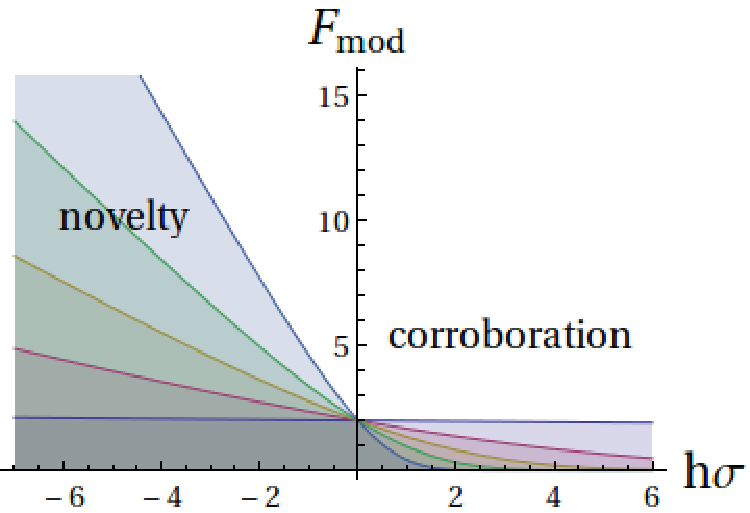
\includegraphics[scale=0.6]{Figures_p/funcmodruido0.png}
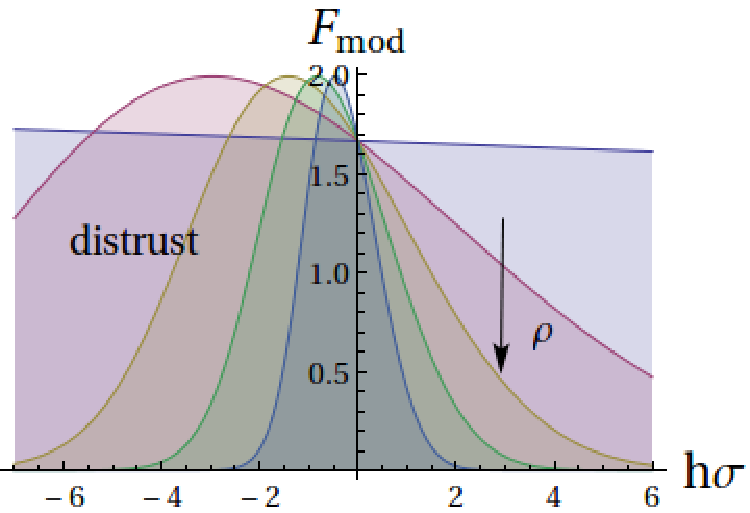
\includegraphics[scale=0.6]{Figures_p/funcmodruido02.png}
\label{fig:fmod}
\end{figure*}

O efeito da aquisição de informação pode ser percebido na figura
\ref{fig:fmod} onde mostramos a função de modulação do aprendizado
Bayesiano em duas situações e para diferentes valores do parâmetro de
socialização ou experiencia moral $\rho$ que cresce no sentido da seta
$\downarrow$. Nessa figura à esquerda é considerado o caso onde não existe
erro de comunicação ($\epsilon = 0$). A medida que o aprendizado ocorre
( $\downarrow$ ) a função de modulação decresce para assuntos em que
existe concordância de opinião ( $z > 0$ ) e aumenta para assuntos em que
existe discordância de opinião ( $z < 0$ ).  Sendo assim, interpretamos que
assuntos que trazem mais informação, que são os assuntos discordantes,
causam mais impacto no aprendizado do agente a medida que o mesmo acumula
experiência. Outro efeito que podemos notar é que para valores pequenos
de $\rho$ o agente terá uma tendência mais corroborativa pois esse dará
bastante importância para classificação de assuntos que estão de acordo
com sua opinião ( $z>0$ ).

Já na figura à esquerda, estamos analisando o caso onde a opinião do parceiro
social é invertida com probabilidade  $\epsilon=0.2$.  O algoritmo Bayesiano
permite incorporar essa informação, o que dá origem a um efeito muito
interessante de desconfiança. Ou seja, se o agente discorda da opinião do
seu parceiro social sobre um assunto e além disso está muito certo da sua
de sua própria opinião ( $z \ll 0$) ele irá aprender pouco com essa nova
informação. É interessante notar que o  efeito de desconfiança fica mais
pronunciado a medida que o agente acumula experiência, ou seja, vemos uma
maior depleção na forma da função de modulação para valores negativos
de $z$ a medida que $\rho$ cresce.

Por fim, é importante fazer um breve comentário sobre uma
simplificação feita para obtermos expressão da função de modulação
\ref{eq:F}. Consideramos a distribuição de probabilidade a posteriori deve
ser projetada sobre famílias de gaussianas com a matriz de covariância
escrita na forma $\bm C = \bm 1 C$, onde $C$ é uma constante e $\bm 1$
é uma matriz identidade. Com essa aproximação implicitamente assumimos
que não existe correlação entre as diferentes dimensões morais ou que
essas dimensões são processadas em partes distintas e pouco conectadas
do cérebro. Apesar  dessa hipótese ser pouco provável do ponto de vista
psicológico e neurológico ela fornecesse uma simplificação que é atrativa
sob a perspectiva matemática e computacional.

\section{Fase 2: Aprendizado da matriz moral}  %#{{{2

Durante a primeira fase o agente aprendeu a aprender, ou seja, nesta fase
ele estabeleceu a estratégia cognitiva para lidar com novas informações.
Na fase 2, assumimos que o agente tem uma estratégia de aprendizado
fixa, o parâmetro mede a complexidade da socialização na primeira fase
se torna independente do tempo $\rho_i(t) = \rho_i$. A validade dessa
hipótese foge do escopo desse trabalho, sendo tema de futuras pesquisas,
no entanto podemos especular que ela tem alguma relação com as fases
de aprendizado de Piaget\citep{Piaget1965}, e (ou) com a dificuldade
da criança e adolescentes tem de se imaginar sobre a perspectiva de
terceiros\cited{Moriguchi2007,Blakemore2008}.

Assumimos ainda que os agentes são influenciados somente por aqueles que
tem o mesmo tipo de estratégia cognitivas, ou seja, $\rho_i = \rho$ para
todo o agente $i$ da sociedade. Apesar de forte, essa hipótese pode ser
justificada pois indivíduos tem a tendencia de considerar mais importantes
as opiniões das pessoas que são parecidas consigo. Essa hipótese equivale
a assumir para o nosso modelo uma espécie de influência informacional
saliente \citep{Abrams1990} através do parâmetro $\rho$ .  No entanto,
os efeitos dessa hipótese não são tão relevantes para os resultados
do modelo pois, como mostramos no apêndice \ref{sec:dd}, uma sociedade de
agentes com diferentes estratégias cognitivas não muda de maneira drástica
o perfil estatístico da opinião de um grupo de agentes que têm a mesma
estratégia cognitiva.

De maneira similar a proposta em \citep{Caticha2011a}, simplificamos a dinâmica
do modelo assumindo que o conjunto de assuntos $\mc X = \{ \bm x_1, \bm
x_2,\ldots,\bm x_P \}$ discutidos pelos agentes podem ser condensados,
ou resumidos, em um assunto médio $\mc Z$,
\[
\mc Z \propto \frac{1}{P}\sum_{\bm x_\mu \in \mc X}\bm x_\mu.
\]
Como o assunto médio captura a essência de todos os assuntos discutidos
na sociedade o chamamos de \textit{Zeitgeist} \footnote{Do alemão
\textit{zeit} significa tempo e \textit{geist} significa espirito ou mente,
o termo \textit{Zeitgeist} é comumente traduzido como espirito do tempo. Para
mais informações a respeito do termo olhar \citep{Forland2008}}. Sem
perda de generalidade o vetor \textit{Zeitgeist} tem uma direção fixa e
é normalizado ($\mc Z=(1,1,1,1,1)/\sqrt{5}$). A opinião de um agente
$i$ em relação ao \textit{Zeitgeist} é definida como, 
\[
h_i = \mc Z \cdot \bm \omega_i.
\]

Na fase 2, as conexões sociais entre os agentes são definidas através de um
grafo $\mc G(\mc V,\mc A)$ onde $\mc V$ é um conjunto de vértices na qual estão
localizados os agentes, e $\mc A$ é o conjunto de arestas, que representa as
conexões sociais entre os agentes propriamente dita. 

A dinâmica do modelo na Fase 2 é similar a uma dinâmica de Metropolis
\citep{Metropolis1953}. Em um tempo de simulação $t$ dois agentes vizinhos
$(i,j)$ são sorteados do conjunto de arestas $\mc A$.  Um dos agentes
vizinhos é sorteado, suponha que seja o agente $i$, para tentar mudar sua
matriz moral $\bm \omega_i$ para uma matriz moral tentativa $\bm \omega_i'$
através da interação social com seus vizinhos\footnote{Fazemos esse
procedimento para o sorteiro do agente pois isso garante que o número
de interações sociais é proporcional ao número conexões sociais do
agente}. A matriz moral tentativa $\bm \omega_i'$ é sorteada uniformemente
de uma hiperesfera unitária de 5 dimensões, e sua aceitação como uma nova
matriz moral pelo agente $i$ ocorre se a energia de interação \footnote{A
expressão da energia de iteração de um agente $i$ com seu vizinho
  $j$ é: \\ $\mc E (h_i,\sigma_j) = \log\left(\epsilon + (1 -
  2\epsilon)\Phi\left(\frac{z}{C}\right)\right)$}
entre o agente e seus vizinhos diminuir. Caso contrario, o agente aceita a
matriz moral tentativa com um probabilidade igual a exponencial de menos a
variação de energia vezes uma constante $\beta$ positiva. Ou seja,
\[
\bm \omega_i \rightarrow \bm \omega_i' \text{ com prob. } 
p = \min\{1,\exp( -\beta \Delta \mc E)\}
\]

Seja $\mc V_i$ a vizinhança do agente $i$, então escrevemos variação de energia
de iteração do agente $i$ em relação aos seus vizinhos como
\[
\Delta \mc E 
= \sum_{k\in\mc V_i } \mc E(h_i',\sigma_k) - \mc E(h_i,\sigma_k)
\]
Chamamos a constante $\beta$ de \textbf{pressão social} ou \textbf{pressão de
pares}. Esse parâmetro tem um papel fundamental na dinâmica, pois ele indica
o nível de flutuação aceitável para as matrizes morais dos agentes. Para
valores de $\beta$ grandes, o agente terá pouca liberdade para mudar sua
matriz moral, já o contrario, para valores de $\beta$ próximos de zero o
agente com grande probabilidade pode assumir uma matriz moral que aumente a
energia de interação com sua vizinhança. De fato, essa interpretação faz
sentido do ponto de vista social, já que é senso comum que sociedades com
grande pressão social não permitem uma grande variação de comportamento.
A fase 2 de nosso modelo é flexível o suficiente para assumirmos que cada
agente tenha uma percepção diferente da pressão social, no entanto,
evidências experimentais\cite{Panagopoulos2011} indicam que as pressão
social não é percebida com grande diferença entre indivíduos numa mesma
sociedade e também não varia muito com o tamanho da comunidade que o
indivíduo está inserido.

\section{Parâmetros de Ordem \\ e transição de fase}  %#{{{2

Duas grandezas importantes para medirmos a dependência das matrizes morais
dos agentes com os parâmetros do modelo, são a média $m$ e variância $v$
das opiniões dos agentes em relação ao \textit{Zeitgeist},
\begin{align}
    m &= \mean{h_i}, \nn
    v &= \mean{(h_i - \mean{h_i})^2};
\end{align}
Essas grandezas são conhecidas como \textit{parâmetros de ordem} já que
as mesmas trazem informação da organização macroscópica do sistema. A
dependência dessas grandezas com a  pressão social $\beta$ e com o medida
de complexidade de socialização $\rho$ pode ser analisado através da figura
\ref{fig:ordem}. Como já foi dito, para valores pequenos do parâmetro $\beta$
existe uma grande dispersão das matrizes morais dos agentes, na figura
\ref{fig:ordem}(b) pode-se observar que a medida que a pressão social
aumenta a variância das opiniões dos agente diminui.

\begin{figure*} 
    \centering
    \begin{subfigure}[]{0.46\textwidth}
        \centering
        \caption{média das opiniões}
        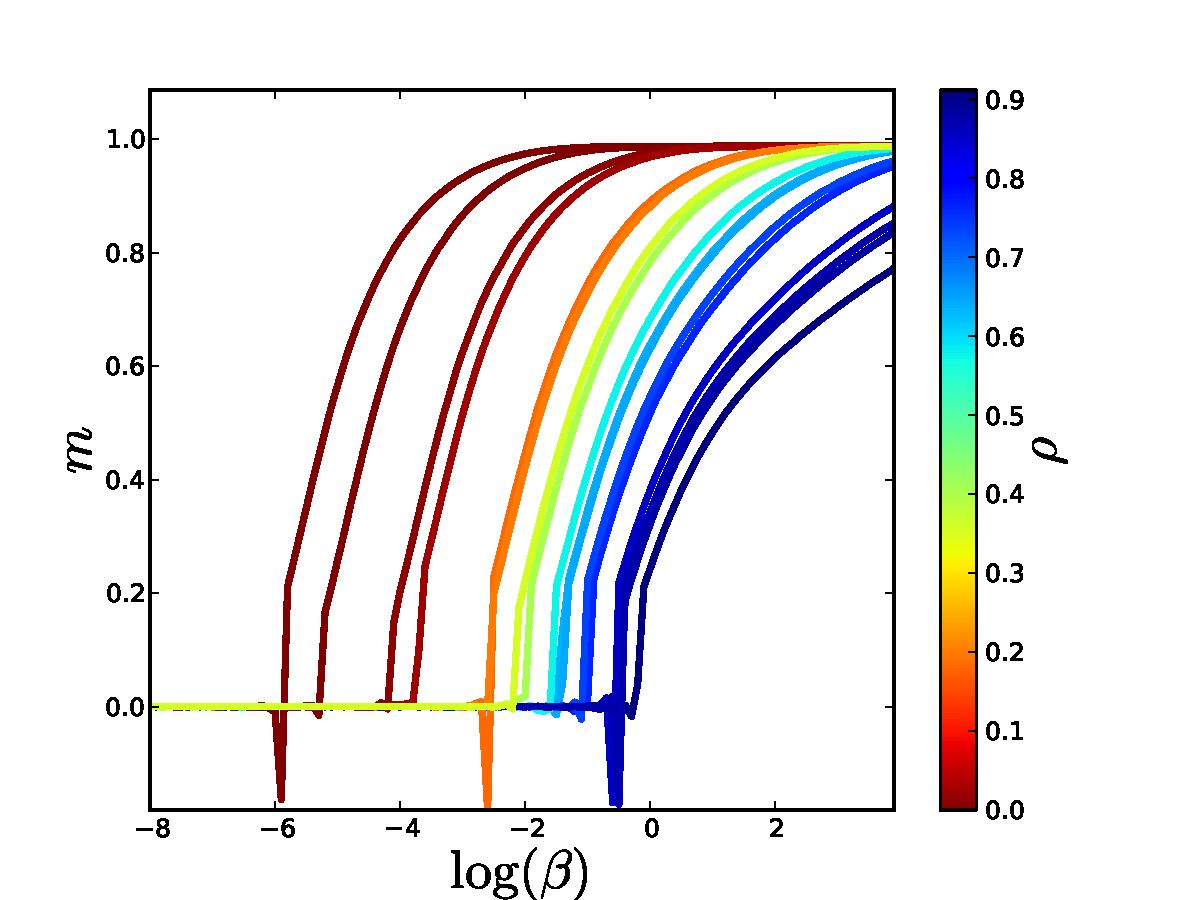
\includegraphics[width = \textwidth]{Figures/mag}
  %\label{fig:Histo_Pol1}
    \end{subfigure}
    \begin{subfigure}[]{0.46\textwidth}
        \centering
        \caption{variância das opiniões}
        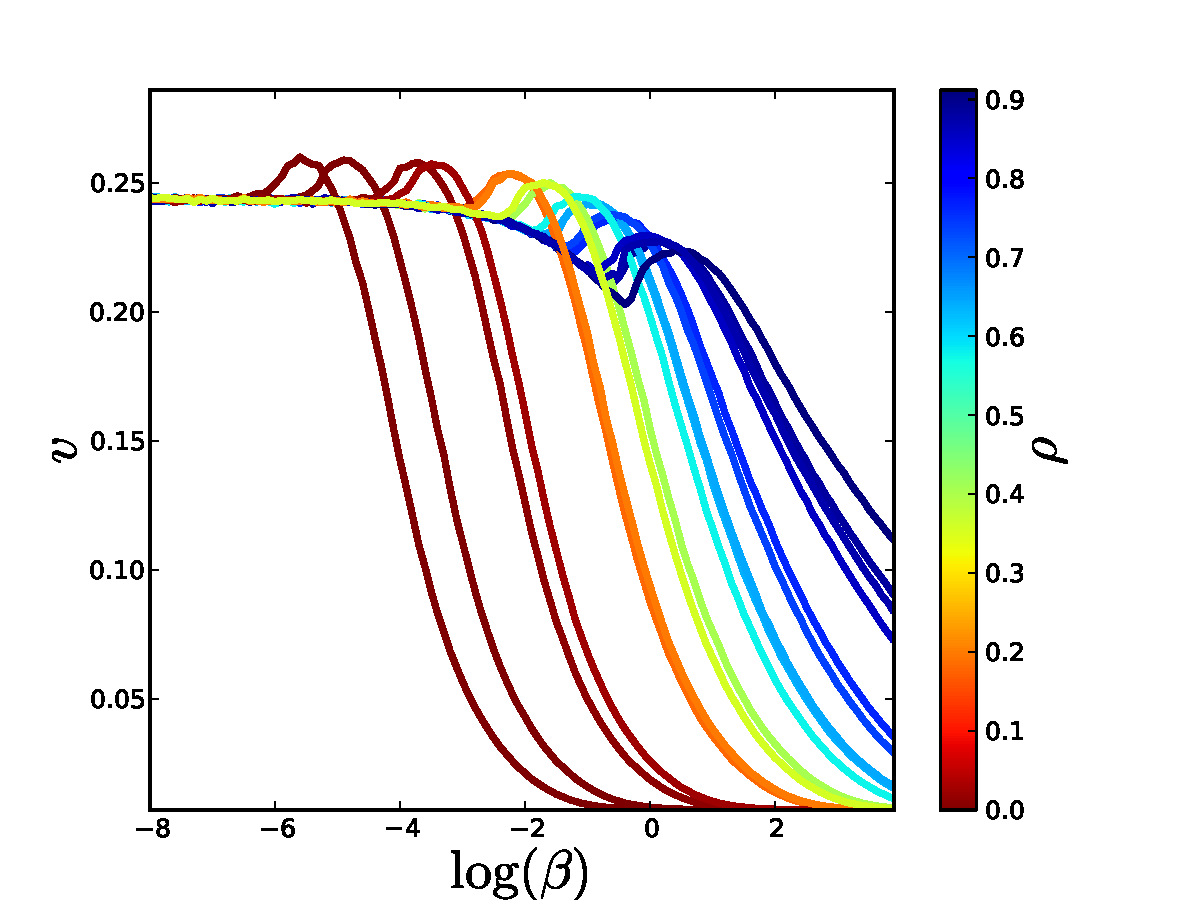
\includegraphics[width = \textwidth]{Figures/sigma}
  %\label{fig:Mag_Pol}
    \end{subfigure}
    \newline
    \caption{
        Dependência dos parâmetros de ordem
    }
    \label{fig:ordem}
\end{figure*}

Um comportamento mais interessante, pode ser notado através da figura
\ref{fig:ordem}(a) onde mostramos a média das opiniões dos agentes em
função de $\beta$. Para valores pequenos de pressão social, a opinião média
dos agentes é nula ($ m = 0$), no entanto, para valores de pressão acima
de um limiar $\beta_c(\rho)$ a as matrizes morais dos agentes se alinham
subitamente na direção do \textit{zeitgeits}, de forma que a opinião
médias do agentes passa a ser maior que zero ($m > 0$).  É importante notar
que a média das opiniões dos agentes muda de maneira abrupta fazendo com
que a derivada da opinião média em relação a pressão social divirja,
o que caracteriza uma espécie \textit{transição de fase} de 2 ordem.

Como em nosso modelo as interações entre os agentes não são simétricas ele não
é um sistema Hamiltoniano, a pesar disso, podemos definir o parâmetro de ordem
\begin{align}
    \chi = \beta\mean{(m - \mean{m})^2},
\end{align}
esse parâmetro é análogo à susceptibilidade magnética do famoso modelo
de Ising, e nada mais é do que a variância da média das opiniões vezes
a pressão social. A utilidade desse parâmetro em nosso modelo  é que
ele caracteriza a transição de fase pelo seu comportamento divergente,
como pode ser notado através da figure \ref{fig:chi}.
\begin{figure}
    \centering
    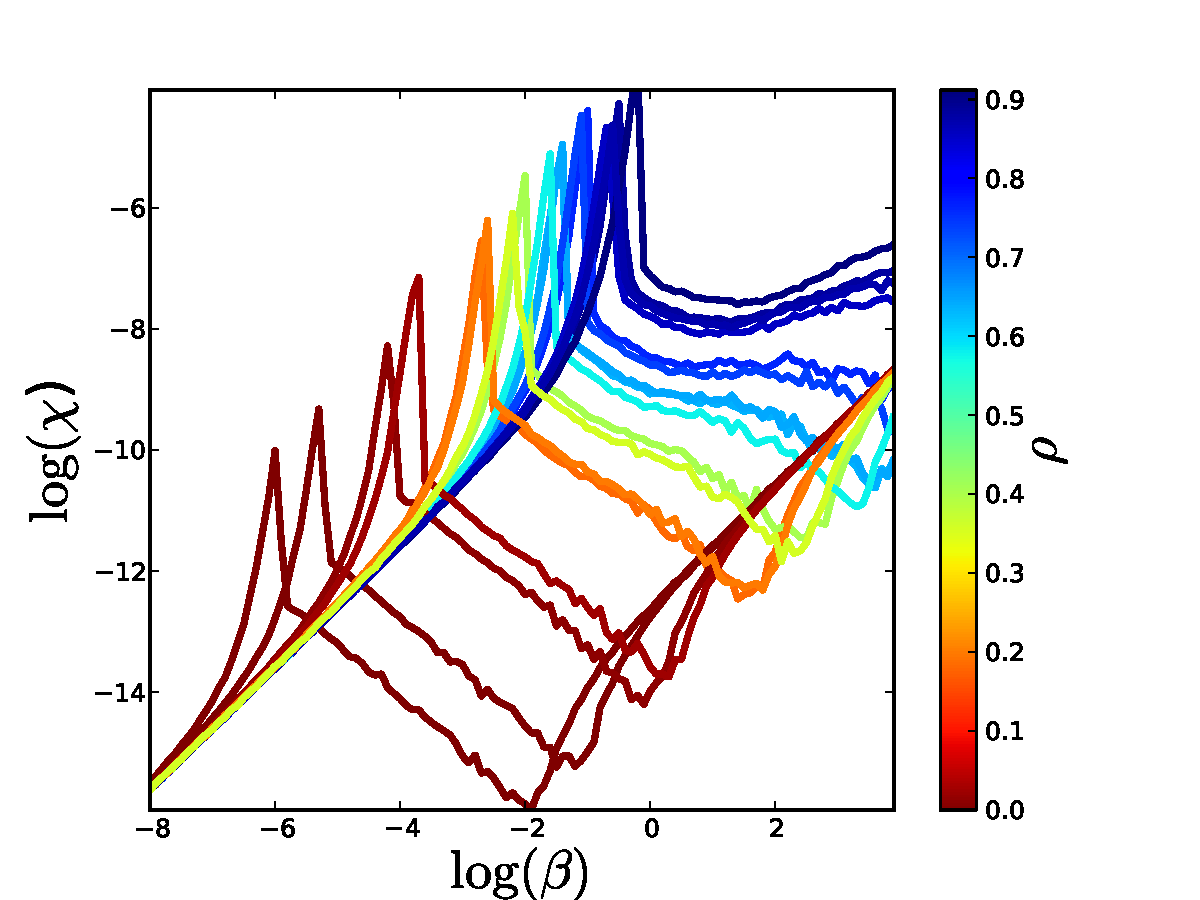
\includegraphics[width = 0.8\textwidth]{Figures/chi}
    \caption{Divergência "susceptibilidade" das opiniões dos agentes.
    Observa-se que essa quantidade diverge em para diferentes 
    valores de $\beta$, caracterizando uma transição de fase.
    }
    \label{fig:chi}
\end{figure}

Por fim, conseguimos notar que a organização dos agentes em torno do
\textit{Zeitgeist} tem uma grande dependência com o parâmetro $\rho$,
observamos que quanto maior é a socialização ( ou quantidade de informação
) que o agente obteve na fase 1, maior o valor da pressão social necessário
para que ocorra transição de fase. Indicamos aos leitores interessados
em fenômenos de transição de fase as referências\cite{Salinas2001,
,Newman1999,Nishimori2011}.

\newpage
\section{Comparação entre dados simulados e experimentais}  %#{{{2

Uma sociedade de agente é caracterizada pelo parâmetro $\beta$ que fornece a
pressão social e pelo parâmetro $\rho$ de socialização.  Assim, para tempos
longos da Fase 2, a sociedade de agentes apresentará uma distribuição de
opiniões sobre o \textit{Zeitgeist} $P_A(h|\rho,\beta)$ estável, apesar das
opiniões individuais dos agentes não serem constantes. Usando um conjunto
de dados contendo aproximadamente 15 mil questionários obtidos através de
\citep{Quest} podemos levantar matrizes morais empíricas normalizadas $\bm
\omega_e$ de indivíduos separados por suas ideologias políticas, numa escala
de $\bm 0$ a $\bm 7$ sendo $\bm 0$ muito liberal e $\bm 7$ muito conservador.

Inferimos o \textit{Zeitgeist} experimental através da matriz moral
média dos indivíduos mais conservadores. Usamos esse procedimento pois,
de acordo com nossa teoria, esperamos que pessoas conservadoras  apresentem
menos dispersão de matrizes morais. Obtemos a informação das opiniões
de cada respondente sobre o \textit{Zeitgeist}, que é dada por $h_e = \bm
\omega_e \cdot \mc Z_e$. Dessa forma, tem-se uma assinatura estatística
dos dados experimentais através de histogramas ou distribuições das
opiniões empíricas dado a ideologia política, $P_E(h|\mathrm{i.p.})$.

Usando a metodologia de \cite{Caticha2011a}, medimos o quão próximo os
histogramas de opiniões feitos por simulação estão dos histogramas
empíricos através da distância definida por 
\begin{equation}
D(\rho,\beta;ip) = \sum_{h\in bins} \left( P_S(h|\rho,\beta) - P_E(h|ip)
\right)^2
\end{equation}
que nada mais é soma da diferença quadrática das frequenciais das
opiniões sobre um conjunto de bins\footnote{o termo bin se refere a um
termo de um conjunto de divisões ou espaçamentos sobre um intervalo}. As
figuras \ref{fig:hist}, \ref{fig:pa-rho} e \ref{fig:diagfase} são obtidas
identificando os histogramas experimentais mais próximos dos simulados com
a restrição de que a distância $D(\rho,\beta;ip)$ seja menor que um certo
valor limiar\footnote{nas figuras apresentas o valor de limiar usado foi 0.1}.

\newpage
\subsection{Dados Experimentais}  %#{{{3

Os dados experimentais foram extraídos do questionário MFQ30\cite{Quest}
e consistem de N = 14250 vetores morais sendo suas componentes relacionadas
com os cinco fundamentos morais num intervalo de [0-5]. Esses dados então são
normalizados para obtermos as matrizes morais experimentais. Na tabela
\ref{tab:data} apresentamos algumas medidas estatísticas relativas as opiniões
experimentais obtidas através do questionário.

\begin{table}
    \begin{tabular}{cccccl}
        \hline
        $ip$ & n & $m_e$& $\mu_e$  &  $\sigma_e$ & \textit{ideologia} \\ \hline
          1  & 2919 & 0.825(5) & 0.837(4) & 0.084(2)  & Muito Liberal \\ 
          2  & 5604 & 0.877(2) & 0.889(2) & 0.069(2)  & Liberal  \\
          3  & 2009 & 0.907(3) & 0.920(3) & 0.063(4)  & Pouco Liberal  \\
          4  & 1448 & 0.932(3) & 0.947(3) & 0.056(4)  & Moderado  \\
          5  & 879  & 0.964(2) & 0.975(2) & 0.035(3)  & Pouco Conservador \\
          6  & 1087 & 0.979(2) & 0.986(1) & 0.026(4)  & Conservador  \\
          7  & 300  & 0.976(4) & 0.987(2) & 0.040(10) & Muito Conservador  \\
       6 + 7 & 1387 & 0.979(2) & 0.987(1) & 0.028(4)  & Conservador  \\ \hline
    \end{tabular}
    \caption{
        retirada de \citep{Caticha2011a}. O termo $ip$ é o índice
        da filiação política dos indivíduos , $m_e$ e $\mu_e$ são
        respectivamente a média e a mediana das opiniões dos respondentes,
        $\sigma_e$ é a variância. Os erro representa com 95\% de confiança do
        bootstrap.
    }
    \label{tab:data}
\end{table}

